% siminos/spatiotemp/chapter/lattProp.tex
% $Author: predrag $ $Date: 2019-05-09 18:30:52 -0400 (Thu, 09 May 2019) $

%%%% input by % siminos/spatiotemp/chapter/catMapLatt.tex %%%%%%%%
\section{Green's function counts all paths}
\label{s-lattProp}

This text is based on
\HREF{http://chaosbook.org/FieldTheory/} {dasbuch/QMlectures/lectQM.tex}.
For reasons unbeknownst to me, it is below the dignity of any cat to work out
any problem in Chaos\-Book, or in the online course, no matter how often I
point out that it is easier to understand what we do for \catlatt\ if you
first work it out for a standard 2\dmn\ lattice.


\bigskip
\noindent
We assume that the state of a particle is specified by its position, and
that it has no further internal degrees of freedom, such as spin or color:
\(
i = (x_1,x_2,\cdots,x_d)
\,.
\)
A particle either does nothing ($s =$~stopping probability) or steps into any
of the \(2d\) neighboring cells ($h =$~stepping probability).
Counting paths on a lattice is a breeze.
Let a particle start in the cell \(i\) and step along until it stops in the
cell \(j\).
The probability of this process is \(h{}^\ell s\), where  \(\ell\) is the
number of steps in the corresponding path. The total probability that a
particle wanders from the $i$th cell and stops in the $j$th cell is the
sum of probabilities associated with all possible paths connecting the
two cells:
\beq
\Delta_{ij} =s \sum_\ell h^\ell N_{ij} (\ell)	
\,,
\ee{(5.1)}
where $N_{ij}(\ell)$ is the number of all paths of length $\ell$
connecting lattice sites $i$ and $j$. In order to compute $N_{ij}(\ell)$,
define a {\stepOp}
    \index{stepping operator}\index{operator!stepping}
\beq
(\hopMat^\mu)_{ij} = \delta_{i+n_\mu , j}
\,, 	
\ee{(5.2)}
where \( n_\mu \) is a unit step in direction \( \mu \).
If a particle is introduced into the $i$th cell by a source
\(
\source_k = \delta_{ik}
\,,
\)
the {\stepOp} moves it into a neighboring cell:
% FieldTheory-p63a.pdf
\[
(\hopMat^\mu \source)_k=\delta_{i+n_\mu , k} \to
%%%%%%%%%%%%%%%%%%%%%%%%%%%%%%%%%%%%%%%%%%%%%%%%%%%%%%%%%%%%%%%%%%
 %% FieldTheory-p63a.pdf
 %% 2013-08-18 dasbuch/book/FigSrc/inkscape/Lesne07Eq5-2a.svg
 ~~~~ \raisebox{-1.5ex}[3.5ex][2.5ex]{
  \setlength{\unitlength}{7ex} %1.00\textwidth}
  \begin{picture}(1,0.47666132)%
    \put(0,0){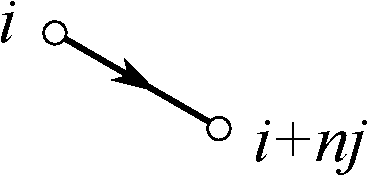
\includegraphics[width=\unitlength]{Lesne07Eq5-2a}}%
    \put(-0.20779928,0.36126749){\color[rgb]{0,0,0}\makebox(0,0)[lb]{\smash{$i$}}}%
    \put(1.08572459,0.03917364){\color[rgb]{0,0,0}\makebox(0,0)[lb]{\smash{$i+n_\mu$}}}%
  \end{picture}%
    }
%%%%%%%%%%%%%%%%%%%%%%%%%%%%%%%%%%%%%%%%%%%%%%%%%%%%%%%%%%%%%%%%%%
%
\]
The operator
\beq
N_{ij} = \sum^d_{\mu=1}
	 [ (\hopMat^\mu)_{ij} + (\hopMat^\mu)_{ji}]
	\,,
% \qquad h_\mu = (h,h, \cdots,h)
\label{(5.3)}
\eeq
generates all steps of length 1:
\[
 \mathbf{N}\, \source = ~~ \raisebox{-3.0ex}[4.5ex][3ex]
    {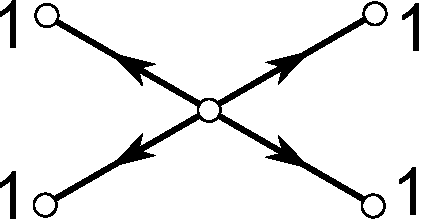
\includegraphics[height=8ex]{Lesne07Eq5-2b}}
%\raisebox{distance}[extend-above][extend-below]
%\mbox{ [FieldTheory-p63b.ps]}
%\,,\qquad
%\mbox{$i$th cell}
%\,.
\]
(The examples are drawn in two dimensions). The paths of length
2 are counted by
\[
\mathbf{N}^2 \source = ~~ \raisebox{-6.0ex}[8.5ex][6.5ex]
    {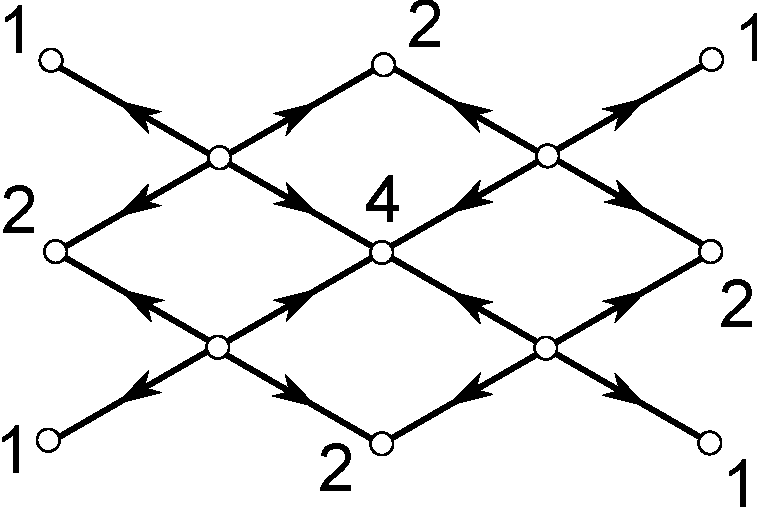
\includegraphics[height=16ex]{Lesne07Eq5-2c}}
%\raisebox{distance}[extend-above][extend-below]
%\mbox{ [FieldTheory-p63c.ps]}
%%\,\,,
\]
There are 4 ways of returning, 2 ways of reaching a diagonal corner, and so on.
Note --and this is the key observation-- that the $k$th
component of the vector $\mathbf{N}^\ell\source $ counts the
number of paths of length \(\ell\) connecting the $i$th and the $k$th
cells. The total probability that the particle stops in the $k$th cell is
given by
\bea
\field_k &=& s \sum_{\ell=0}^\infty
		 h^\ell \mathbf{N}^\ell_{kj} \source_{j}
	\,,\qquad
\field \,=\, \frac{s}{ 1- h \mathbf{N}} \source
\,.
\label{(5.4)}
\eea
%\PC{}{insert:
%Interpreting $\field$ as a field is consistent with the previous
%definition of a free field, equations
%\refeq{(2.22)} and \refeq{(2.25)}.
%	 }
The value of the field	$\field_k$ at a space point
$k$ measures the
probability of observing the particle introduced into the system
by the source $\source$. The Euclidean free scalar particle propagator
--or Green's function--
\refeq{(5.1)} is given by
\beq
\Delta_{ij} =  \left(\frac{s}{ 1- h \mathbf{N}}\right)_{ij}
\,.
\label{(5.5)}
\eeq
Consider a smooth function $\field(x)$ evaluated on a
$d$-dimensional lattice
\beq
\field_\ell
=
\field(x)
    \,,\qquad \qquad x = a\ell= \mbox{lattice point}
    \,,\quad \ell \in {\bf Z}^d
\,,
\ee{LattField}
where $a$ is the lattice spacing. Each set of values of $\field(x)$ (a
vector $\field_\ell$) is a possible lattice configuration. Assume the
lattice is hyper-cubic, and let
$
\hat{n}_\mu
    \in
\left\{\hat{n}_1, \hat{n}_2, \cdots , \hat{n}_d\right\}
$
be the unit lattice cell vectors pointing along the $d$ positive
directions.
The {\em lattice derivative} is then
    \index{lattice!derivative}\index{derivative, lattice}
%$ \left|\hat{n}_\mu\right| = 1$
\beq
(\partial_\mu \field)_\ell
        =
    \frac{ \field(x+a{\hat{n}_\mu}) - \field(x)
        }{a}
        =
    \frac{ \field_{\ell+{\hat{n}_\mu}} - \field_\ell
        }{a }
\,.
\ee{latticePartDer}
The lattice derivative as a
linear operator, constructed from the {\em {\stepOp}} in the direction
$\mu$
\index{stepping operator}\index{operator!stepping}
\beq
\left(\hopMat_\mu\right)_{\ell j}=\delta_{\ell+{\hat{n}_\mu},j}
\,.
\ee{hopMat}
In practice, the lattice will be a finite
$d$-dimensional hyper-cubic lattice
\beq
\field_\ell
=
\field(x)
    \,,\qquad \qquad x = a\ell= \mbox{lattice point}
    \,,\quad \ell \in \left({\bf Z}/N\right)^d
\,,
\ee{LattFieldN}
where $a$ is the lattice spacing and there are $N^d$ points in all. For a
hyper-cubic lattice the translations in different directions commute,
$\hopMat_\mu \hopMat_\nu = \hopMat_\nu \hopMat_\mu$, so it is sufficient to
understand the action of \refeq{hopMat} on a 1-dimensional periodic lattice,
on which the {\stepOp} is an [$N\!\times\!N$] `upper shift' cyclic
permutation matrix
\index{cyclic!permutation matrix}
\beq
\hopMat
=\begin{bmatrix}   0    &  1    &        &        &   &  \cr
                  &  0    &   1    &        &   &  \cr
                  &       &   0    &  1     &   &  \cr
                  &       &        &   & \ddots &  \cr
                  &       &        &        & 0 & 1 \cr
             1    &       &        &        &   & 0
         \end{bmatrix}
\,,
\ee{hopMatrix}
with `1' in the lower left corner assuring periodicity.
Applied to the lattice configuration
$\field=(\field_1,\field_2, \cdots, \field_N)$,
the {\stepOp} translates the configuration by one site,
$\hopMat \field=(\field_2,\field_3, \cdots, \field_N,\field_1)$.
Its transpose translates the configuration the other way, so the transpose is
also the inverse,
\( %beq
\hopMat^{-1}=\hopMat^{T}
\,.
\) %ee{TransHop}
The partial lattice derivative \refeq{latticePartDer} can now be
written as a multiplication by a matrix:
\[
\partial_\mu \field_\ell =
    \frac{1}{a}\left(\hopMat_\mu  - \unit \right)_{\ell j} \field_j
\,.
\]
In the 1-dimensional case the [$N\!\times\!N$] matrix representation of
this lattice derivative is:
\beq
%\frac{1}{a}(\hopMat - \unit)
\partial
= \frac{1}{a}
 \begin{bmatrix}  -1    &  1    &        &     &        &      \cr
                  & -1    &   1    &     &        &      \cr
                  &       &  -1    &  1  &        &      \cr
                  &       &        &     & \ddots &      \cr
                  &       &        &     &        &    1 \cr
             1    &       &        &     &        &   -1
         \end{bmatrix}
\,.
\ee{LattDerMat}
The symmetric (self-adjoint) combination
$\Box = - \partial^T\partial$
\index{lattice!Laplacian}\index{Laplacian!lattice}
    \PC{}{recheck the signs!}
\bea
\Box
%\hopMat^{-1}\partial^2
    &=& - \frac{1}{a^2} \sum_{\mu=1}^d
  \left(\hopMat^{-1}_\mu  - \unit \right)
  \left(\hopMat_\mu  - \unit \right)
    =
- \frac{2}{a^2}
    \sum_{\mu=1}^d
 \left(\unit - \frac{1}{2} (\hopMat^{-1}_\mu + \hopMat_\mu) \right)
\continue
    &=& \frac{1}{a^2}\left(\mathbf{N} -2d \unit\right)
\label{Lat-Lap}
\eea
is the {\em lattice Laplacian}.
In the 1-dimensional case the [$N\!\times\!N$] matrix representation of
the lattice Laplacian is:
\beq
\Box
    % \hopMat^{-1}\partial^2
=
\frac{1}{a^2}
 \begin{bmatrix}  -2    &  1    &        &     &        &    1 \cr
             1    & -2    &   1    &     &        &      \cr
                  &  1    &  -2    &  1  &        &      \cr
                  &       &   1    &     & \ddots &      \cr
                  &       &        &     &        &    1 \cr
             1    &       &        &     &    1   &   -2
         \end{bmatrix}
\,.
\ee{LattLap}
The lattice Laplacian measures the second variation of a field
$\field_\ell$ across three neighboring sites: it is spatially
\emph{non-local}.
The Euclidean ``free scalar particle propagator'' \refeq{(5.5)}, or the
``Green's function'' can thus be written as
\beq
\Delta =  \frac{1}{ \unit-  \frac{a^2h}{s}\Box}
\,.
\label{(5.5a)}
\eeq
In  \catlatt\ we are not thinking of a continuum, so we set
the lattice spacing to $a=1$.

Now, were there even a single alert cat out there (and there should not be a
dry eye in the feline audience at this moment), it would not escape her
attention that \refeq{Lat-Lap} looks very much like the \catlatt\
eq.~\refeq{LinearConnPC}:
\beq
(\Box_{zz'} +2d \unit)_{zz'} x_{z'} =  s x_{z} + \m_z
    \,, \qquad
  x_{z} \in  \mathbb{T}^{1}
    \,, \;\;
  m_{z} \in \A
    \,, \;\;
  z\in \integers^{d}
\,.
\ee{LaplCounts}
The operator $\mathbf{N} = s\unit$ of \refeq{(5.3)} generates all steps of
length 1. More precisely, all ways of staying at the site $x_{z}$. So now we
know what $s$ does in the \catlatt\ equation~\refeq{LinearConnPC}: it counts
in how many ways we can get from $x_{z}$ to $x_{z}$, with some extra
`particles' subtracted by the source terms $\m_z$. How ``subtracted?'' Well,
Boris did not like \PV\rf{PerViv} convention (too many
``-''s!), so in \refeq{LinearConnPC} $\m_z$ shows up with the wrong sign.

\section{Trace formula for counting periodic points}
\label{sect:Helmoltz}
% not in ChaosBook as of 2018-08-10

The total number of points periodic with period $\ell$ is
given by $\tr N(\ell) = \sum_j N(\ell)_{jj}$. For an infinite lattice
this is infinite, just because the number of pints $j$ is infinite,
but as all points are equivalent, it suffices
to count all periodic orbits going through a given marked point,
let's say site $0$ at the origin, $N(\ell)_{00}$.
All possible paths returning to site $0$ can be
collected in generating function (see \refeq{(5.1)}):
\beq
\left.\Delta\right|_{00} = \sum_\ell z^\ell N(\ell)_{00}
  = \left.\frac{1}{ 1- z \mathbf{N}}\right|_{00}	
\,,
\ee{(5.1)00}
where the number of periodic points $N_{00}(\ell)$ is the number of all
periodic paths of length $\ell$ that include lattice site $0$.
As the one-step generator $\mathbf{N}$ is a matrix, its
eigenvalues provide explicit formula for $N(\ell)_{00}$.

This formula, and all above formulas of this section generate and count
single-particle walks on the lattice.

However, this is not the counting problem we want to solve
in the case of \catlatt.
Instead, we need to determine $N^{[\speriod{}\times\period{}]}$, the
number of ``periodic points,'' or doubly-periodic \twot\ states $\Xx$
over the discrete 2-torus $T^2_{[\speriod{}\times\period{}]}$ (or $\R =
\R^{[\speriod{}\times\period{}]}$) compatible with the 2\dmn\  damped
Poisson equation \refeq{catLattPC}. If $\speriod{},\period{}$ are both
primes, each periodic point $\Xx$ belongs to a group orbit of
$\speriod{}\period{}$ periodic points equivalent up to a spacetime
translation, hence ``periodic points'' $\Xx$, and a prime \po\ is the
group orbit of $\Xx$, \ie, the set of all $\Xx$ obtained by spacetime
translations.

We should convince ourselves that $N^{[\speriod{}\times\period{}]}$ is
given by the ``trace'' of the damped Poisson equation Green's function,
and that the equation itself yields the $N^{[\speriod{}\times\period{}]}$
formula \refeq{HLnumberOfPeriodicOrbits9}.
\PC{2018-08-10}{
Notation $N^{[\speriod{}\times\period{}]}$ is experimental.
    }
